% Created by tikzDevice version 0.8.1 on 2015-01-12 15:12:44
% !TEX encoding = UTF-8 Unicode
% Drawing Rectangle from x0 = -0.000000, y0 = 0.000000 to x1 = 289.080000, y1 = 289.080000
% Beginning new tikzpicture 'page'
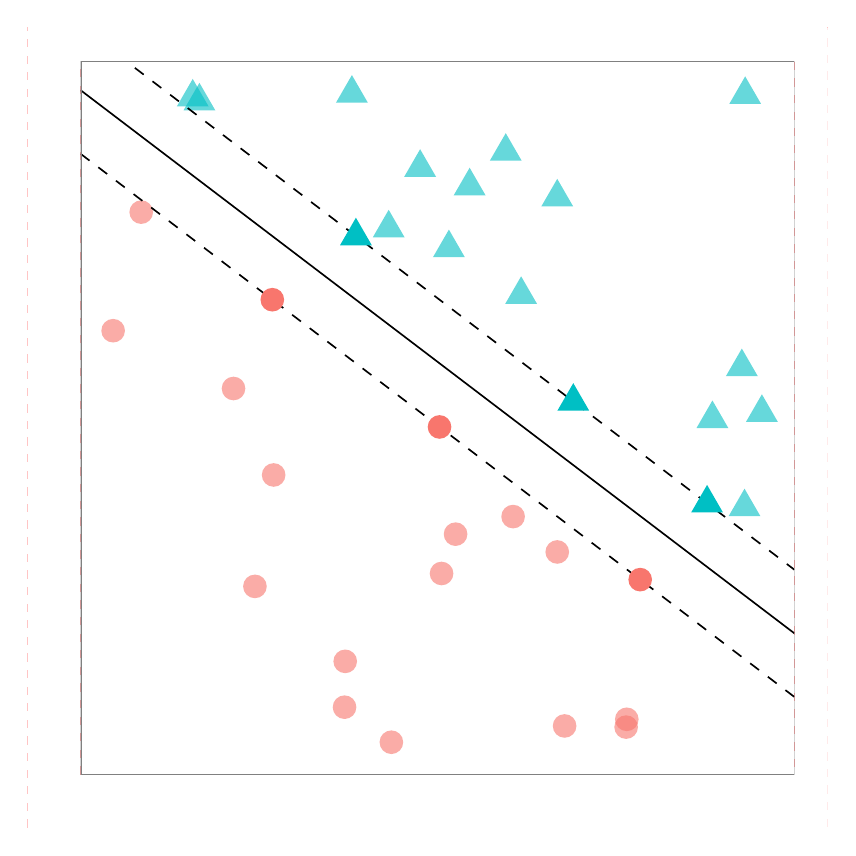
\begin{tikzpicture}[x=1pt,y=1pt]
\definecolor{fillColor}{RGB}{255,255,255}
\path[use as bounding box,fill=fillColor,fill opacity=0.00] (0,0) rectangle (289.08,289.08);
\begin{scope}
\path[clip] (  0.00,  0.00) rectangle (289.08,289.08);
\path[draw=red,very thick,dashed] (  0.00,  0.00) rectangle (289.08,289.08);
\definecolor{drawColor}{RGB}{255,255,255}
\definecolor{fillColor}{RGB}{255,255,255}

\path[draw=drawColor,line width= 0.6pt,line join=round,line cap=round,fill=fillColor] ( -0.00,  0.00) rectangle (289.08,289.08);
\end{scope}
% Drawing Rectangle from x0 = 19.158189, y0 = 19.158189 to x1 = 277.035000, y1 = 277.035000
\begin{scope}
\path[clip] ( 19.16, 19.16) rectangle (277.04,277.03);
\path[draw=red,very thick,dashed] ( 19.16, 19.16) rectangle (277.04,277.03);
\definecolor{fillColor}{RGB}{255,255,255}

\path[fill=fillColor] ( 19.16, 19.16) rectangle (277.03,277.03);
% Drawing Circle at x = 154.622062, y = 106.056512, r = 4.267913
\definecolor{fillColor}{RGB}{248,118,109}

\path[fill=fillColor,fill opacity=0.60] (154.62,106.06) circle (  4.27);
% Drawing Circle at x = 175.406885, y = 112.405282, r = 4.267913

\path[fill=fillColor,fill opacity=0.60] (175.41,112.41) circle (  4.27);
% Drawing Circle at x = 191.358028, y = 99.634396, r = 4.267913

\path[fill=fillColor,fill opacity=0.60] (191.36, 99.63) circle (  4.27);
% Drawing Circle at x = 216.251478, y = 36.338631, r = 4.267913

\path[fill=fillColor,fill opacity=0.60] (216.25, 36.34) circle (  4.27);
% Drawing Circle at x = 30.879862, y = 179.575760, r = 4.267913

\path[fill=fillColor,fill opacity=0.60] ( 30.88,179.58) circle (  4.27);
% Drawing Circle at x = 194.016551, y = 36.759871, r = 4.267913

\path[fill=fillColor,fill opacity=0.60] (194.02, 36.76) circle (  4.27);
% Drawing Circle at x = 114.744205, y = 60.099534, r = 4.267913

\path[fill=fillColor,fill opacity=0.60] (114.74, 60.10) circle (  4.27);
% Drawing Circle at x = 149.546698, y = 91.852348, r = 4.267913

\path[fill=fillColor,fill opacity=0.60] (149.55, 91.85) circle (  4.27);
% Drawing Circle at x = 41.030590, y = 222.420523, r = 4.267913

\path[fill=fillColor,fill opacity=0.60] ( 41.03,222.42) circle (  4.27);
% Drawing Circle at x = 131.420400, y = 30.879862, r = 4.267913

\path[fill=fillColor,fill opacity=0.60] (131.42, 30.88) circle (  4.27);
% Drawing Circle at x = 88.884018, y = 127.453968, r = 4.267913

\path[fill=fillColor,fill opacity=0.60] ( 88.88,127.45) circle (  4.27);
% Drawing Circle at x = 114.502521, y = 43.542980, r = 4.267913

\path[fill=fillColor,fill opacity=0.60] (114.50, 43.54) circle (  4.27);
% Drawing Circle at x = 82.116867, y = 87.186336, r = 4.267913

\path[fill=fillColor,fill opacity=0.60] ( 82.12, 87.19) circle (  4.27);
% Drawing Circle at x = 216.493162, y = 39.157305, r = 4.267913

\path[fill=fillColor,fill opacity=0.60] (216.49, 39.16) circle (  4.27);
% Drawing Circle at x = 74.382979, y = 158.685155, r = 4.267913

\path[fill=fillColor,fill opacity=0.60] ( 74.38,158.69) circle (  4.27);
% Starting Polygon
\definecolor{fillColor}{RGB}{0,191,196}

\path[fill=fillColor,fill opacity=0.60] (152.21,216.11) --
	(157.95,206.15) --
	(146.46,206.15) --
	cycle;
% End Polyline
% Starting Polygon

\path[fill=fillColor,fill opacity=0.60] (265.31,156.60) --
	(271.06,146.65) --
	(259.57,146.65) --
	cycle;
% End Polyline
% Starting Polygon

\path[fill=fillColor,fill opacity=0.60] ( 62.06,269.15) --
	( 67.81,259.19) --
	( 56.31,259.19) --
	cycle;
% End Polyline
% Starting Polygon

\path[fill=fillColor,fill opacity=0.60] (259.03,122.50) --
	(264.78,112.54) --
	(253.28,112.54) --
	cycle;
% End Polyline
% Starting Polygon

\path[fill=fillColor,fill opacity=0.60] (172.75,250.96) --
	(178.50,241.01) --
	(167.00,241.01) --
	cycle;
% End Polyline
% Starting Polygon

\path[fill=fillColor,fill opacity=0.60] (247.43,154.37) --
	(253.18,144.41) --
	(241.68,144.41) --
	cycle;
% End Polyline
% Starting Polygon

\path[fill=fillColor,fill opacity=0.60] (259.27,271.48) --
	(265.02,261.52) --
	(253.52,261.52) --
	cycle;
% End Polyline
% Starting Polygon

\path[fill=fillColor,fill opacity=0.60] ( 59.64,270.56) --
	( 65.39,260.61) --
	( 53.89,260.61) --
	cycle;
% End Polyline
% Starting Polygon

\path[fill=fillColor,fill opacity=0.60] (141.81,245.16) --
	(147.56,235.20) --
	(136.06,235.20) --
	cycle;
% End Polyline
% Starting Polygon

\path[fill=fillColor,fill opacity=0.60] (130.45,223.27) --
	(136.20,213.31) --
	(124.71,213.31) --
	cycle;
% End Polyline
% Starting Polygon

\path[fill=fillColor,fill opacity=0.60] (159.70,238.46) --
	(165.45,228.51) --
	(153.95,228.51) --
	cycle;
% End Polyline
% Starting Polygon

\path[fill=fillColor,fill opacity=0.60] (191.36,234.45) --
	(197.11,224.50) --
	(185.61,224.50) --
	cycle;
% End Polyline
% Starting Polygon

\path[fill=fillColor,fill opacity=0.60] (178.31,199.23) --
	(184.06,189.27) --
	(172.56,189.27) --
	cycle;
% End Polyline
% Starting Polygon

\path[fill=fillColor,fill opacity=0.60] (258.06,173.13) --
	(263.81,163.17) --
	(252.31,163.17) --
	cycle;
% End Polyline
% Starting Polygon

\path[fill=fillColor,fill opacity=0.60] (117.16,271.95) --
	(122.91,261.99) --
	(111.41,261.99) --
	cycle;
% End Polyline
% Drawing line from x1 =    19.1582, y1 =   266.4560 to x2 =   277.0350, y2 =    70.2328
\definecolor{drawColor}{RGB}{0,0,0}

\path[draw=drawColor,line width= 0.6pt,line join=round] ( 19.16,266.46) -- (277.04, 70.23);
% Drawing line from x1 =    19.1582, y1 =   243.4683 to x2 =   277.0350, y2 =    47.2451

\path[draw=drawColor,line width= 0.6pt,dash pattern=on 4pt off 4pt ,line join=round] ( 19.16,243.47) -- (277.04, 47.25);
% Drawing line from x1 =    19.6362, y1 =   289.0800 to x2 =   277.0350, y2 =    93.2205

\path[draw=drawColor,line width= 0.6pt,dash pattern=on 4pt off 4pt ,line join=round] ( 19.64,289.08) -- (277.04, 93.22);
% Drawing Circle at x = 88.400650, y = 190.780418, r = 4.267913
\definecolor{fillColor}{RGB}{248,118,109}

\path[fill=fillColor] ( 88.40,190.78) circle (  4.27);
% Drawing Circle at x = 148.821646, y = 144.804975, r = 4.267913

\path[fill=fillColor] (148.82,144.80) circle (  4.27);
% Drawing Circle at x = 221.326842, y = 89.634443, r = 4.267913

\path[fill=fillColor] (221.33, 89.63) circle (  4.27);
% Starting Polygon
\definecolor{fillColor}{RGB}{0,191,196}

\path[fill=fillColor] (118.61,220.41) --
	(124.36,210.45) --
	(112.86,210.45) --
	cycle;
% End Polyline
% Starting Polygon

\path[fill=fillColor] (197.16,160.64) --
	(202.91,150.68) --
	(191.41,150.68) --
	cycle;
% End Polyline
% Starting Polygon

\path[fill=fillColor] (245.50,123.86) --
	(251.24,113.90) --
	(239.75,113.90) --
	cycle;
% End Polyline
% Drawing Rectangle from x0 = 19.158189, y0 = 19.158189 to x1 = 277.035000, y1 = 277.035000
\definecolor{drawColor}{gray}{0.50}

\path[draw=drawColor,line width= 0.6pt,line join=round,line cap=round] ( 19.16, 19.16) rectangle (277.03,277.03);
\end{scope}
\end{tikzpicture}
% Calculated string width 0 times
